\documentclass[
%% TIKZ_CLASSOPTION %%
tikz
]{standalone}
\usepackage{amsmath}
\usetikzlibrary{matrix}
%% EXTRA_TIKZ_PREAMBLE_CODE %%
\begin{document}
%% TIKZ_CODE %%
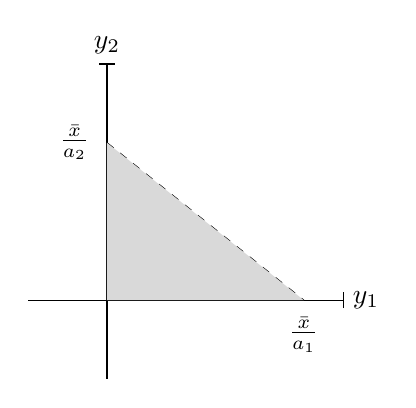
\begin{tikzpicture}
    % Eje x
    \draw (-1,0) -- (3,0) node[right] {$y_1$};
    \draw (0,-0.1) -- (0,0.1);
    \draw (3,-0.1) -- (3,0.1);
    
    % Etiquetas en el eje x
    \node[below] at (2.5,-0.1) {$\frac{\bar x}{a_1}$};
    
    % Eje y
    \draw (0,-1) -- (0,3) node[above] {$y_2$};
    \draw (-0.1,0) -- (0.1,0);
    \draw (-0.1,3) -- (0.1,3);
    
    % Etiquetas en el eje y
    \node[left] at (-0.1,2) {$\frac{\bar x}{a_2}$};
    
    % Recta
    \draw[dashed] (0,2) -- (2.5,0);
    
    % Triángulo
    \fill[gray!30] (0,0) -- (0,2) -- (2.5,0) -- cycle;


    
\end{tikzpicture}
\end{document}
